\documentclass[a4paper]{article}
\usepackage[utf8]{inputenc}
\usepackage[russian,english]{babel}
\usepackage[T2A]{fontenc}
\usepackage[left=10mm, top=20mm, right=18mm, bottom=15mm, footskip=10mm]{geometry}
\usepackage{indentfirst}
\usepackage{amsmath,amssymb}
\usepackage[italicdiff]{physics}
\usepackage{graphicx}
\usepackage{amsmath}
\usepackage[utf8]{inputenc}\newcommand{\approxtext}[1]{\ensuremath{\stackrel{\text{#1}}{\approx}}}
\graphicspath{{images/}}
\DeclareGraphicsExtensions{.pdf,.png,.jpg}
\usepackage{wrapfig}

\usepackage{caption}
\captionsetup[figure]{name=Рисунок}
\captionsetup[table]{name=Таблица}
  
\title{\textbf{Вопрос по выбору}}
\date{}
\author{Котляров Михаил, Б01-402}


\begin{document}

\maketitle
\begin{center}\textbf{ Траектории небесных тел вокруг Солнца в зависимости от гравитационного закона}\end{center}

\section*{Аннотация}
В данной работе исследуются траектории движения небесных тел вокруг Солнца в зависимости от вида силы гравитационного взаимодействия и других параметров.

\section{Сила, подчиняющаяся закону Ньютона}
Для начала выведем настоящие траектории небесных тел. Примем, что на планету со стороны Солнца действует сила тяготения, подчиняющаяся закону Ньютона. Найдем. движение планеты под действием такой силы. Массу Солнца будем считать бесконечно большой по сравнению с массой планеты. Возьмем полярную систему координат $(r, \varphi)$,
полюс которой поместим в центре Солнца. Скорость планеты $v$ можно разложить на радиальную скорость $v_r = \dot{r}$ и перпендикулярную к ней азимутальную скорость $v_\varphi = r  \dot{\varphi}$. Получаем $v^2 = {\dot{r}}^2 +r^2  {\dot{\varphi}}^2$. Законы сохранения энергии и момента
импульса планеты запишем в виде
\begin{equation} \tag{1}
\frac{1} {2} ({\dot{r}}^2 +r^2  {\dot{\varphi}}^2) - \frac{GM}{r} = \varepsilon,
\end{equation}
\begin{equation} \tag{2}
\frac{1} {2} r^2 \dot{\varphi} = \sigma,
\end{equation}
где М — масса Солнца, $\varepsilon$ — полная энергия планеты, приходящаяся на единицу ее массы, $\sigma$ — секториальная скорость, остающаяся постоянной во время движения. Для нахождения уравнения траектории планеты исключим время. Считая $r$ функцией $\varphi$, имеем $ \dot{r} = \frac{dr}{d\varphi}\dot{\varphi}$. Подставляя это значение в уравнение (1) и исключая $\dot{\varphi}$ с помощью уравнения 2, получим
\begin{equation} \tag{3}
(\frac{1}{r^2}\frac{dr}{d\varphi})^2 + \frac{1}{r^2} = \frac{1}{2\sigma^2}(\varepsilon + \frac{GM}{r}).
\end{equation}
Далее решаем дифференциальное уравнение. Приводим к виду
\[
\int{\frac{dr}{r\sqrt{\varepsilon r^2 + GMr - 2\sigma^2}}} = \int{\frac{\pm d\varphi}{\sqrt{2}\sigma}},
\]
получаем
\[
\frac{\arcsin{(\frac{GMr-4\sigma^2}{r\sqrt{8\sigma^2 \varepsilon+G^2 M^2}})}}{\sqrt{2}\sigma} = C \pm \frac{\varphi} {\sqrt{2}\sigma}.
\]
Окончательно
\begin{equation} \tag{4}
r(\varphi) = \frac{\frac{4\sigma^2} {GM}}{1 - \sqrt{1 + \frac{8\varepsilon\sigma^2}{G^2 M^2}} \sin{(\varphi_0 + \varphi)}}.
\end{equation}
Это — уравнение конического сечения с эксцентриситетом $e = \sqrt{1 + \frac{8\varepsilon\sigma^2}{G^2 M^2}}$.
Если $\varepsilon < 0$, то $ e < 1$ (эллипс); если $\varepsilon = 0$, то  $ e = 1$ (парабола); если $\varepsilon > 0$,
то $ e > 1$ (гипербола). 

Чтобы построить реальную траекторию Земли вокруг Солнца, найдем и вычислим необходимые величины.  Масса Солнца $M = 1,98892\cdot10^{30}  \text{ кг}$, Скорость Земли в перигелии (на самом деле можно в любой точке) $v_{п} = 30,27  \frac{\text{км}}{c}$, расстояния от Солнца до перигелия и апогелия соответственно равны $a_{\text{п}} = 147,09 \text{ млн. км}$, $a_{\text{а}} = 152,1 \text{ млн. км}$, период обращения вокруг Солнца $T = 365,256 \text{ суток}$, Гравитационная постоянная $G = 6,67 \cdot 10^{-11}  \frac {\text{Н} \cdot \text{м}^2}{\text{кг}^2} $. С помощью следующих формул вычисляем:
\[
a = \frac{a_{\text{а}} + a_{\text{п}}}{2} \stackrel{}{\approx} 149,595 \text{ млн. км},
\]

\[
\sigma = \frac{1}{2} r^2 \dot{\varphi}= \frac{1}{2} \frac{L}{m} = \frac{1}{2} v_{\perp} r = \frac{1}{2} v_{\text{п}} a_{\text{п}} \stackrel{}{\approx} 2,23 \cdot 10^{15}  \frac{\text{м}^2}{c},
\]

\[
\varepsilon = \frac{v_{\text{п}}^2}{2} - \frac{GM}{a_{\text{п}}} \stackrel{}{\approx} -4,44 \cdot 10^8 \text{ Дж}.
\]
В итоге уравнение движения Земли
\[
r(\varphi) = \frac{1,5 \cdot 10^{11}}{1-0,0167\cos(\varphi)}
\]

\begin{figure}[h!]
    \centering
    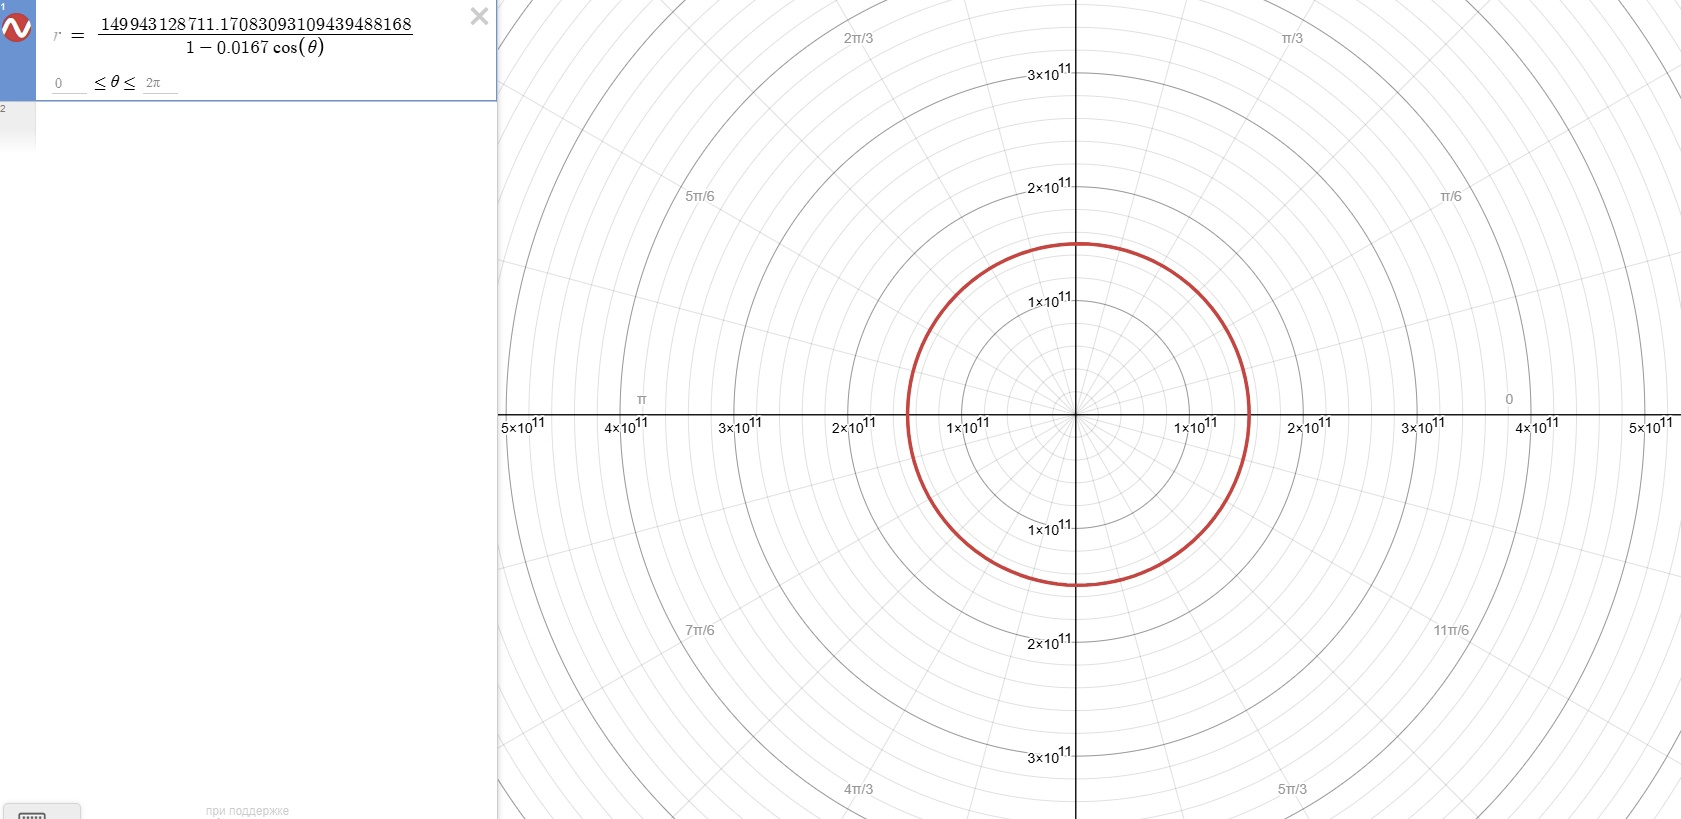
\includegraphics[width=0.9\textwidth]{Ellipse1.jpg}
    \caption{Траектория Земли вокруг Солнца.}
\end{figure}

\begin{figure}[h!]
    \centering
    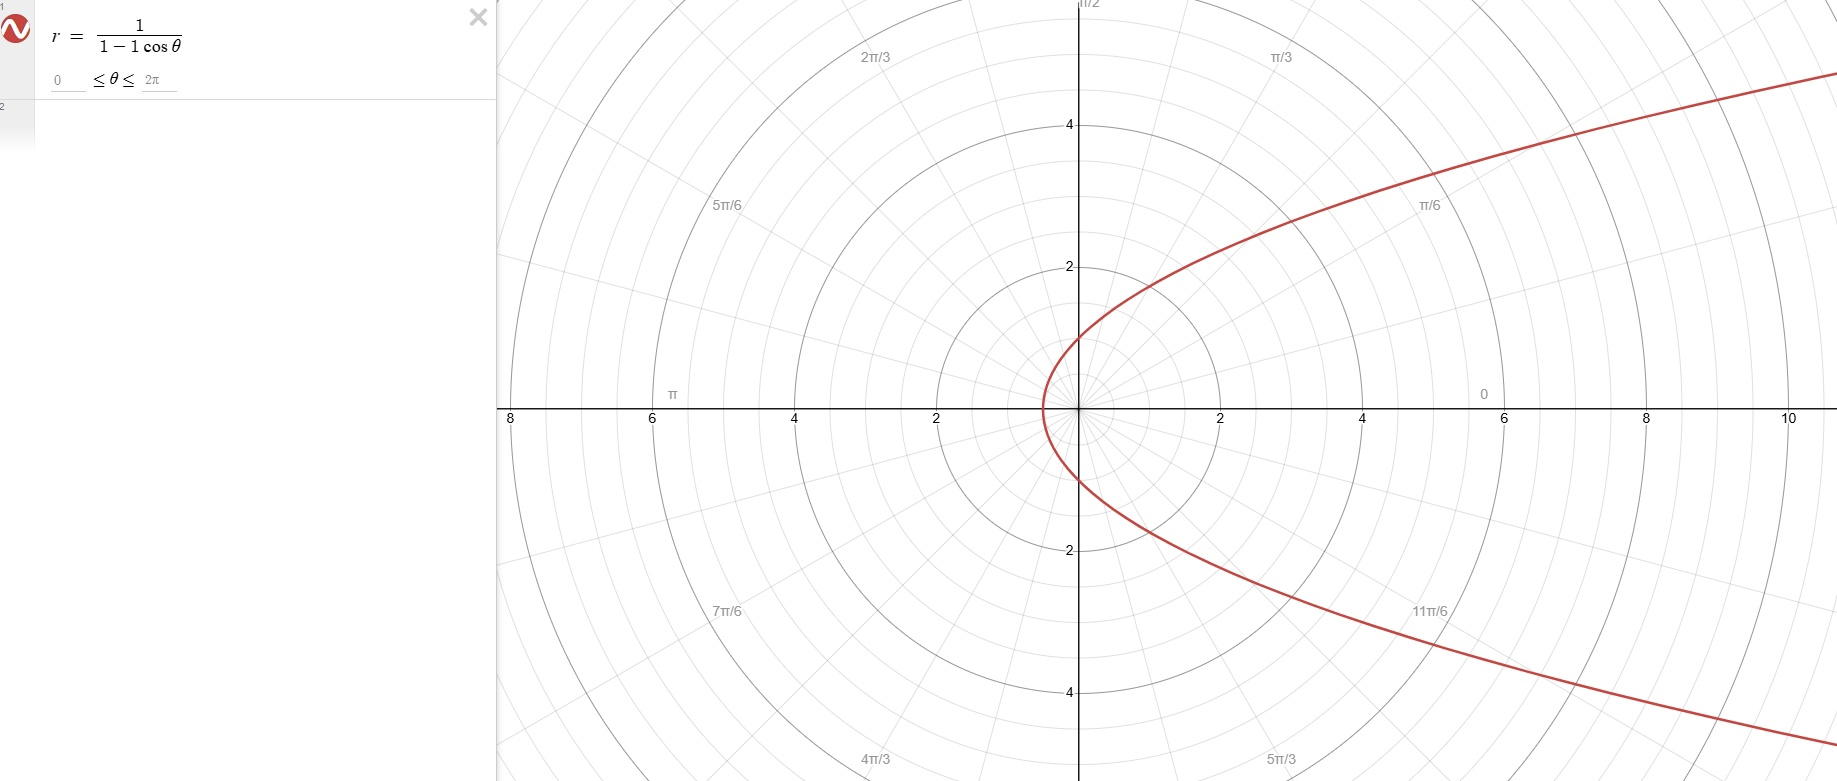
\includegraphics[width=0.9\textwidth]{Parabola1.jpg}
    \caption{Траектория тела при $e = 1$.}
    \clearpage
\end{figure}
\clearpage
\begin{figure}[h!]
    \centering
    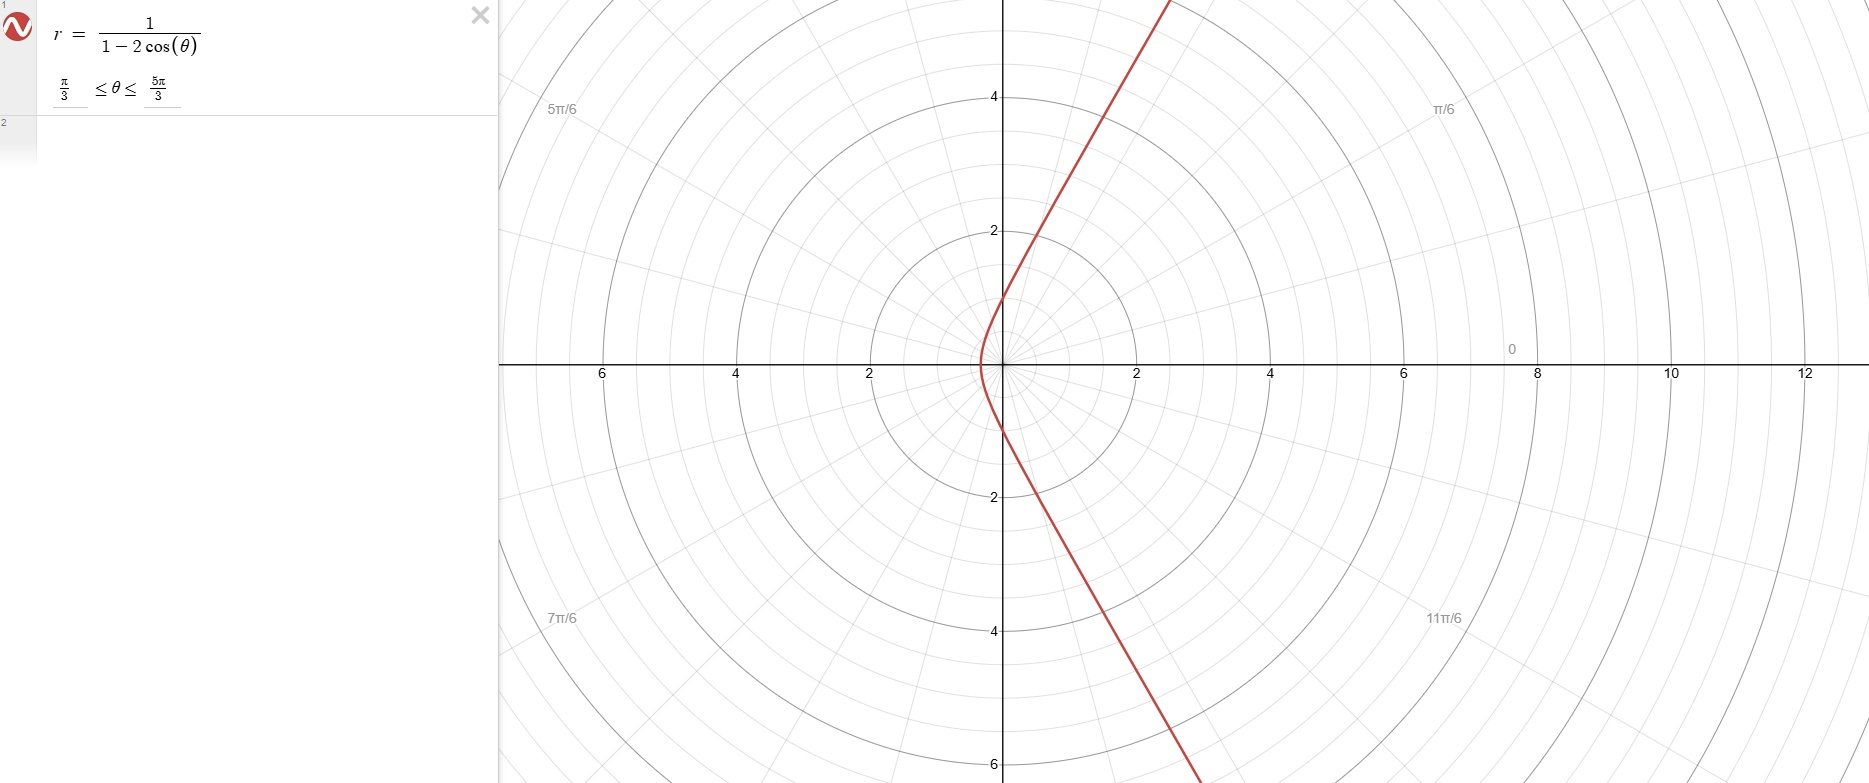
\includegraphics[width=0.9\textwidth]{Hyperbola1.jpg}
    \caption{Траектория тела при $e > 1$.}
\end{figure}

\section{Сила, обратно пропорциональная кубу расстояния}
Теперь представим, что закон Ньютона выглядит следующим образом
\[
\vec{F} = -\frac{GMm} {r^4} \vec{r}
\]
или через модуль силы
\[
F = \frac{GMm} {r^3},
\]
где $G$ - новая Гравитационная постоянная с размерностью $[G] = \frac{\text{Н} \cdot \text{м}^3}{\text{кг}^2}$. Предлагаю исследовать, какой была бы траектория небесных тел, движущихся под действием такой силы.
Потенциальная энергия гравитационного взаимодействия
\[
E_{\text{п}} = \int_{r}^{\infty}{(\vec{F} , d\vec{r})} = -\int_{r}^{\infty}{\frac{GMm}{r^3} \, dr} = -\frac{2GMm}{r^2}.
\]
Теперь решим получившееся дифференциальное уравнение
\[
(\frac{1}{r^2}\frac{dr}{d\varphi})^2 + \frac{1}{r^2} = \frac{1}{2\sigma^2}(\varepsilon + \frac{2GM}{r^2}),
\]

\[
\int{\frac{dr}{r\sqrt{\varepsilon r^2 + 2GM - 2\sigma^2}}} = \int{\frac{\pm d\varphi}{\sqrt{2}\sigma}},
\]

\[
\frac{\arctg{(\frac{\sqrt{\varepsilon r^2-2\sigma^2+2GM}}{\sqrt{2\sigma^2-2GM}})}}{\sqrt{\sigma^2-GM}} = C \pm \frac{\varphi} {\sigma}.
\]
Итого
\begin{equation} \tag{5}
r(\varphi) =\pm \frac{\sqrt{\frac{2(\sigma^2-GM)}{\varepsilon}}}{\cos(\varphi_0 \pm \frac{\sqrt{\sigma^2-GM}}{\sigma}\varphi)}.
\end{equation}
При $\frac{\sqrt{\sigma^2-GM}}{\sigma} \longrightarrow 0 $ траектория закручивается в окружность, при $\frac{\sqrt{\sigma^2-GM}}{\sigma} \longrightarrow 1 $ траектория слабо отклоняется. Это логично с точки зрения параметров движения. При больших значениях секториальной скорости ($\sigma^2 >> GM$) тело пролетает мимо объекта, к которому оно притягивается. При малых - "падает" на него, закручиваясь по спирали.
Если бы Земля двигалась по такому закону, то при настоящих параметрах ($\sigma, G, M, \varepsilon$) она пролетела мимо Солнца практически без отклонений (поскольку $\sigma^2 >> GM$).

\begin{figure}[h]
    \centering
    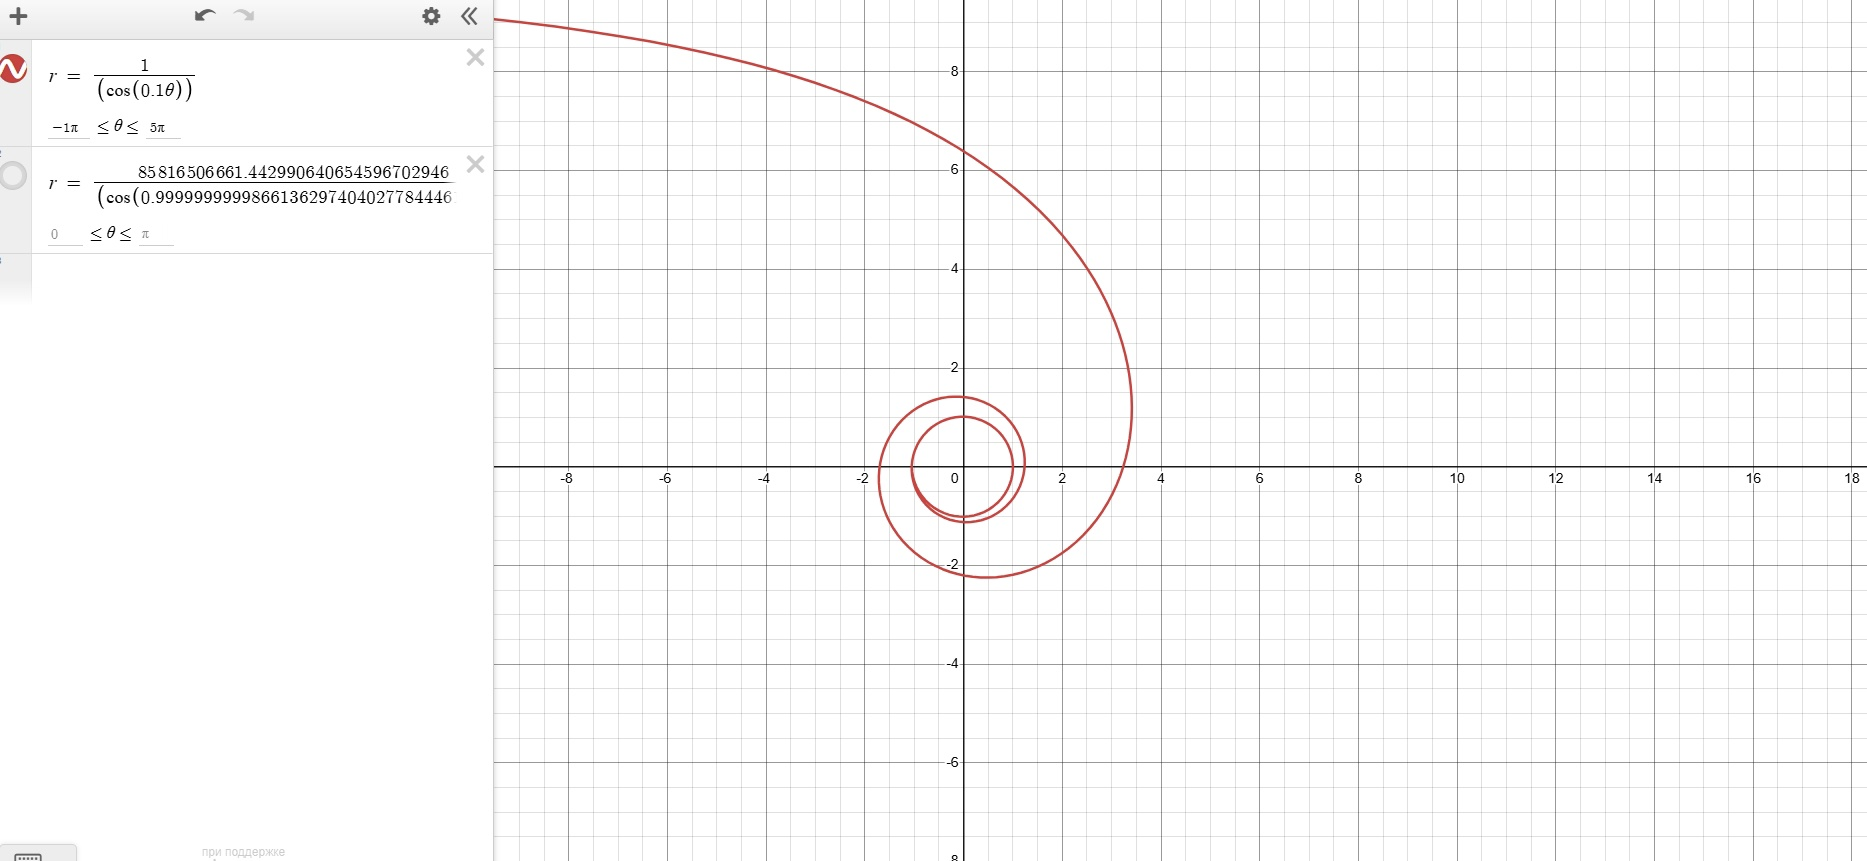
\includegraphics[width=0.7\textwidth]{Graphic2_1.jpg}
    \caption{Траектория 1.}
\end{figure}

\begin{figure}[h]
    \centering
    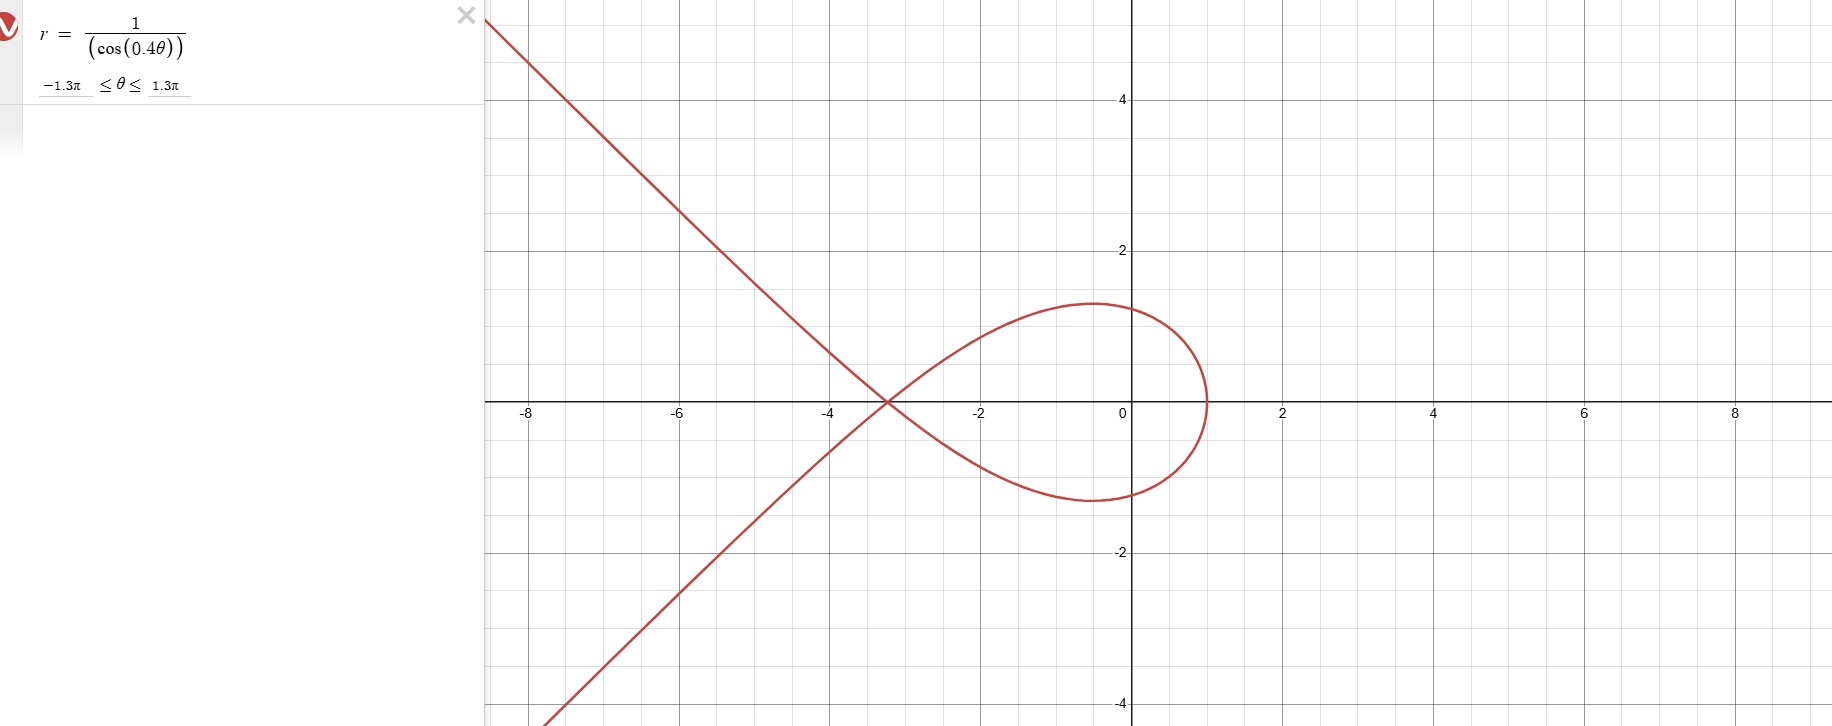
\includegraphics[width=0.7\textwidth]{Graphic2_2.jpg}
    \caption{Траектория 2.}
\end{figure}

\begin{figure}[h]
    \centering
    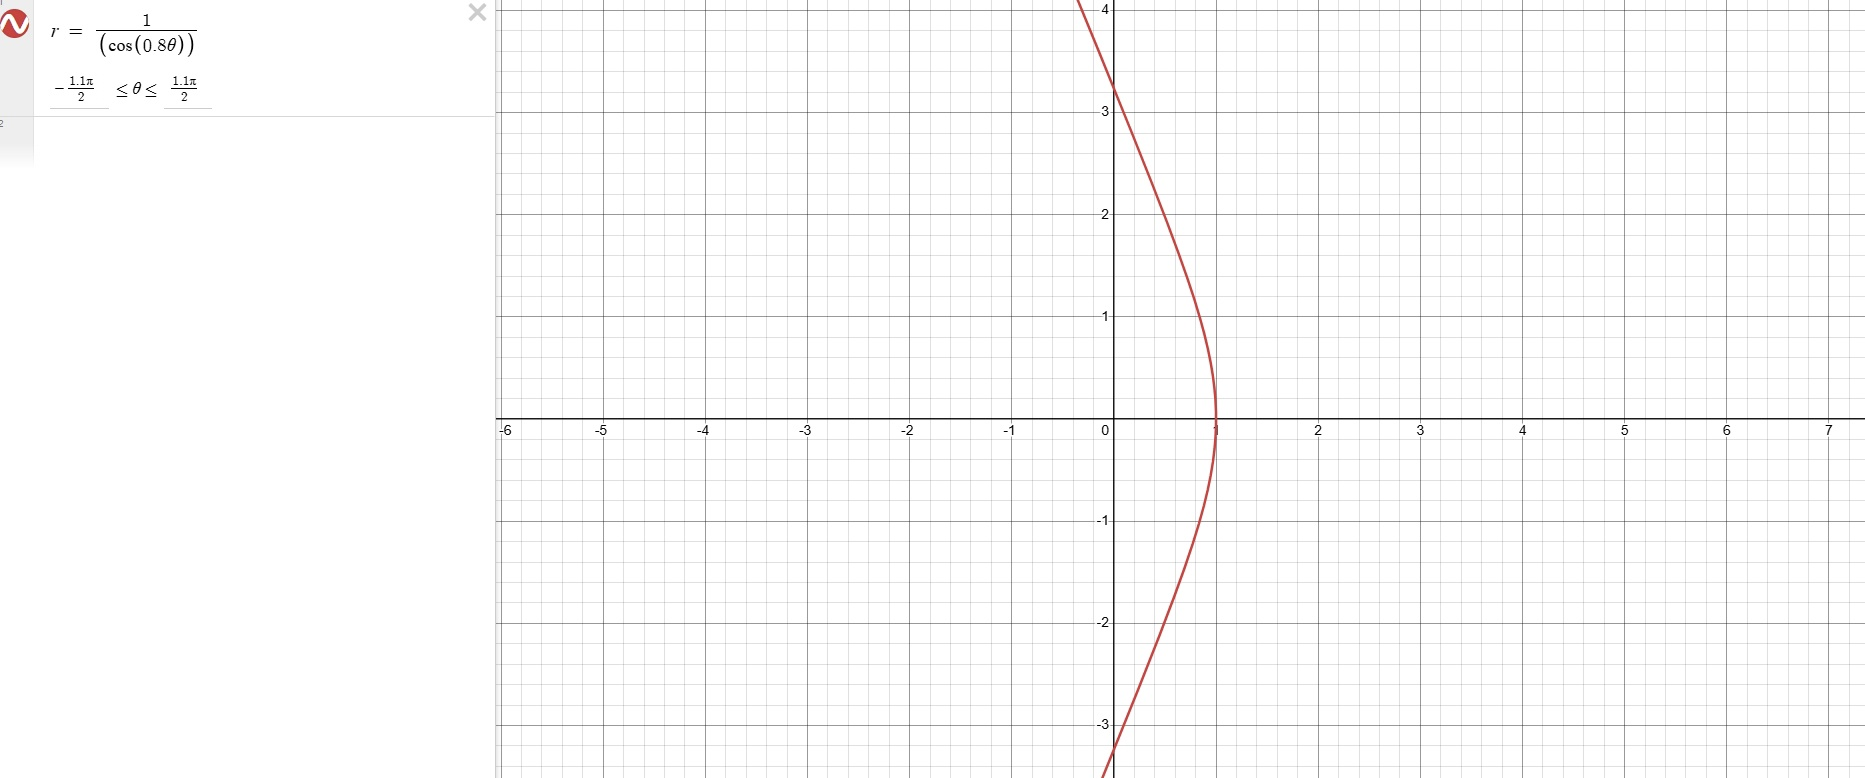
\includegraphics[width=0.7\textwidth]{Graphic2_3.jpg}
    \caption{Траектория 3.}
\end{figure}
\clearpage

Построим приблизительную зависимость (без точных коэффициентов) $\varepsilon(r)$, чтобы проанализировать тип траектории (финитная или инфинитная).
\[
\frac{{v_{r}}^2}{2} + \frac{2\sigma^2}{r^2} - \frac{2GM}{r^2} = \varepsilon.
\]
Получится уравнение гиперболы. Поэтому траектория всегда будет инфинитной.
\begin{figure}[h]
    \centering
    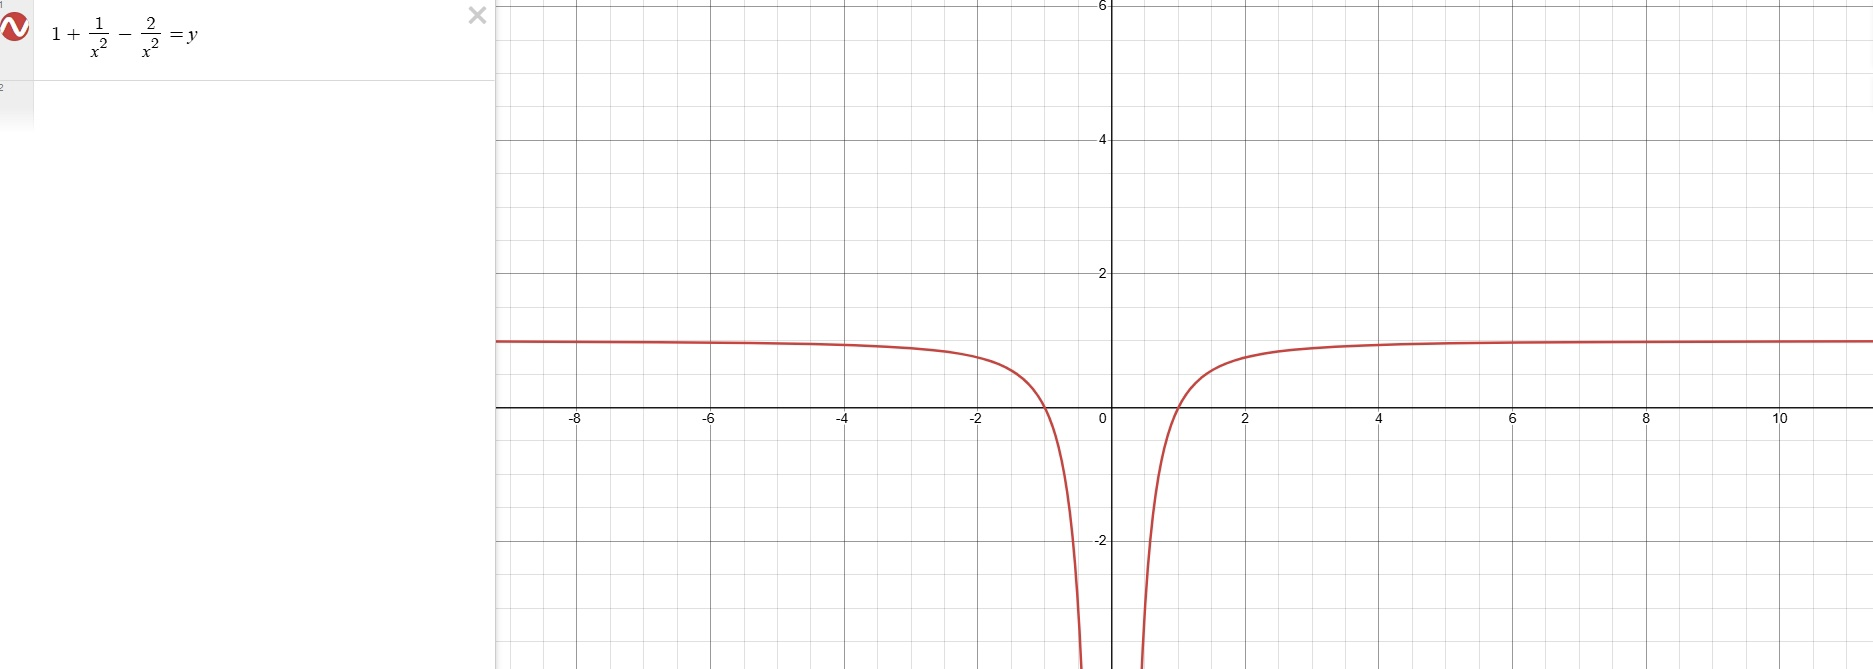
\includegraphics[width=0.9\textwidth]{Finit1.jpg}
    \caption{График $\varepsilon(r) $ №1.}
\end{figure}

\section{Сила, прямо пропорциональная расстоянию в первой степени}
Теперь проделаем те же операции, но для силы по закону 
\[
\vec{F} = -GMm \vec{r}.
\]
 $[G] = \frac{\text{Н}}{\text{м} \cdot \text{кг}^2}$.
Потенциальная энергия гравитационного взаимодействия
\[
E_{\text{п}} = \int_{r}^{\infty}{(\vec{F} , d\vec{r})} = -\int_{r}^{\infty}{GMmr \, dr} = 2GMm r^2.
\]
Решим получившееся дифференциальное уравнение
\[
(\frac{1}{r^2}\frac{dr}{d\varphi})^2 + \frac{1}{r^2} = \frac{1}{2\sigma^2}(\varepsilon - 2GMr^2),
\]

\[
\int{\frac{dr}{r\sqrt{\varepsilon r^2 - 2GMr^4 - 2\sigma^2}}} = \int{\frac{\pm d\varphi}{\sqrt{2}\sigma}},
\]

\[
\frac{\arcsin{(\frac{\varepsilon r^2 - 4\sigma^2}{\sqrt{\varepsilon^2-16GM\sigma^2} r^2})}}{2\sqrt{2}\sigma} = C \pm \frac{\varphi} {\sqrt{2}\sigma}.
\]
Итого
\begin{equation} \tag{6}
r(\varphi) = \frac{\frac{2\sigma}{\varepsilon}}{\sqrt{1-\sqrt{1-\frac{16GM\sigma^2}{\varepsilon^2}}\sin{(\varphi_0 + 2\varphi)}}}.
\end{equation}
Проверим область определения получившейся функции. Внешний корень всегда определен, поскольку 
\\$\sqrt{1-\frac{16GM\sigma^2}{\varepsilon^2}}< 1$, $\abs{\sin{(\varphi_0 + 2\varphi)}} < 1$. Проверим внутренний корень:
\[
1-\frac{16GM\sigma^2}{\varepsilon^2}  \geqslant 0,
\]

\begin{equation} \tag{7}
\abs{\varepsilon}  \geqslant 4\sqrt{GM}\sigma.
\end{equation}

$\varepsilon$ представим в виде

\begin{equation} \tag{8}
\varepsilon =  \frac{{v_r}^2} {2} + \frac{2\sigma^2}{r^2} + 2GMr^2.
\end{equation}

Очевидно, что данная величина всегда положительна. Поэтому раскрываем модуль и подставляем (8) в (7)
\[
\frac{{v_r}^2} {2} + \frac{2\sigma^2}{r^2} + 2GMr^2  \geqslant 4\sqrt{GM}\sigma.
\]

\[
\frac{{v_r}^2} {2} + 2(\frac{\sigma} {r} - \sqrt{GM}r)^2  \geqslant 0 , \text{ при любых значениях величин}.
\]

Поэтому функция удовлетворяет любым параметрам.
Перейдем к анализу параметров зависимости. Для удобства перепишем в следующем виде

\[
r(\varphi) = \frac{p}{\sqrt{1-e\sin{(\varphi_0 + 2\varphi)}}},
\]

где $p = \frac{2\sigma}{\varepsilon}, e = \sqrt{1-\frac{16GM\sigma^2}{\varepsilon^2}}$. Если перейти в ДПСК, то получится уравнение кривой 4-го порядка из-за возникающих модулей при извлечения из-под корня. Но если раскрыть, получится эллипс. Параметр $p$ как и в других зависимостях имеет размерность радиуса и отвечает за масштаб траектории. Когда параметр $e \longrightarrow 0$, траектория превращается в эллипс, когда $e \longrightarrow 1$, траектория стремится к прямой (бесконечно вытянутый эллипс). Это можно получить и с точки зрения физики. Когда $\sigma$ или $v_r$, или $v$ в целом очень большие, когда тело находится вблизи, то оно пролетает мимо (об этом свидетельствует, что $\frac{16GM\sigma^2}{\varepsilon^2} \longrightarrow 0$). Или если оно находится на большом расстоянии от объекта, то у него большая потенциальная энергия, которая перейдет в кинетическую. Если наоборот $v_r = 0$, то траектория может превратиться в окружность, если $\frac{\sigma}{r} = \sqrt{GM}r$ или $r = \sqrt[\leftroot{0}\uproot{1}4]{\frac{\sigma^2}{GM}}$.

Из-за большой потенциальной энергии на расстоянии от Солнца Земля двигалась бы практически по прямой (при настоящих параметрах).

\begin{figure}[h]
    \centering
    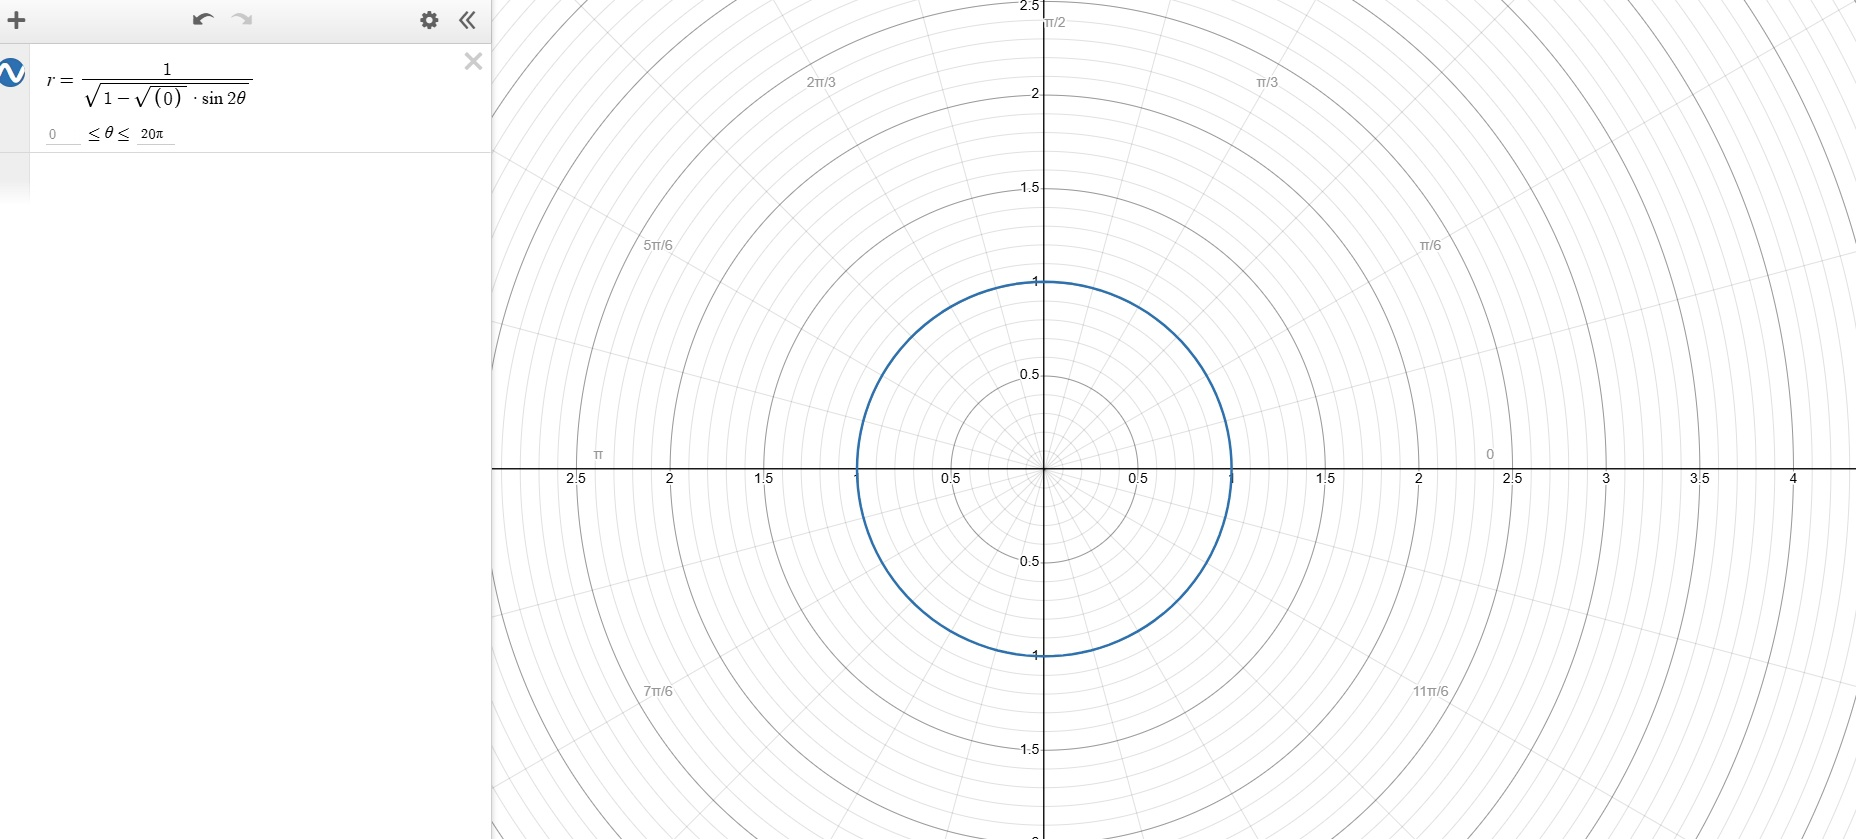
\includegraphics[width=0.7\textwidth]{Graphic3_1.jpg}
    \caption{Траектория 1.}
\end{figure}

\begin{figure}[h]
    \centering
    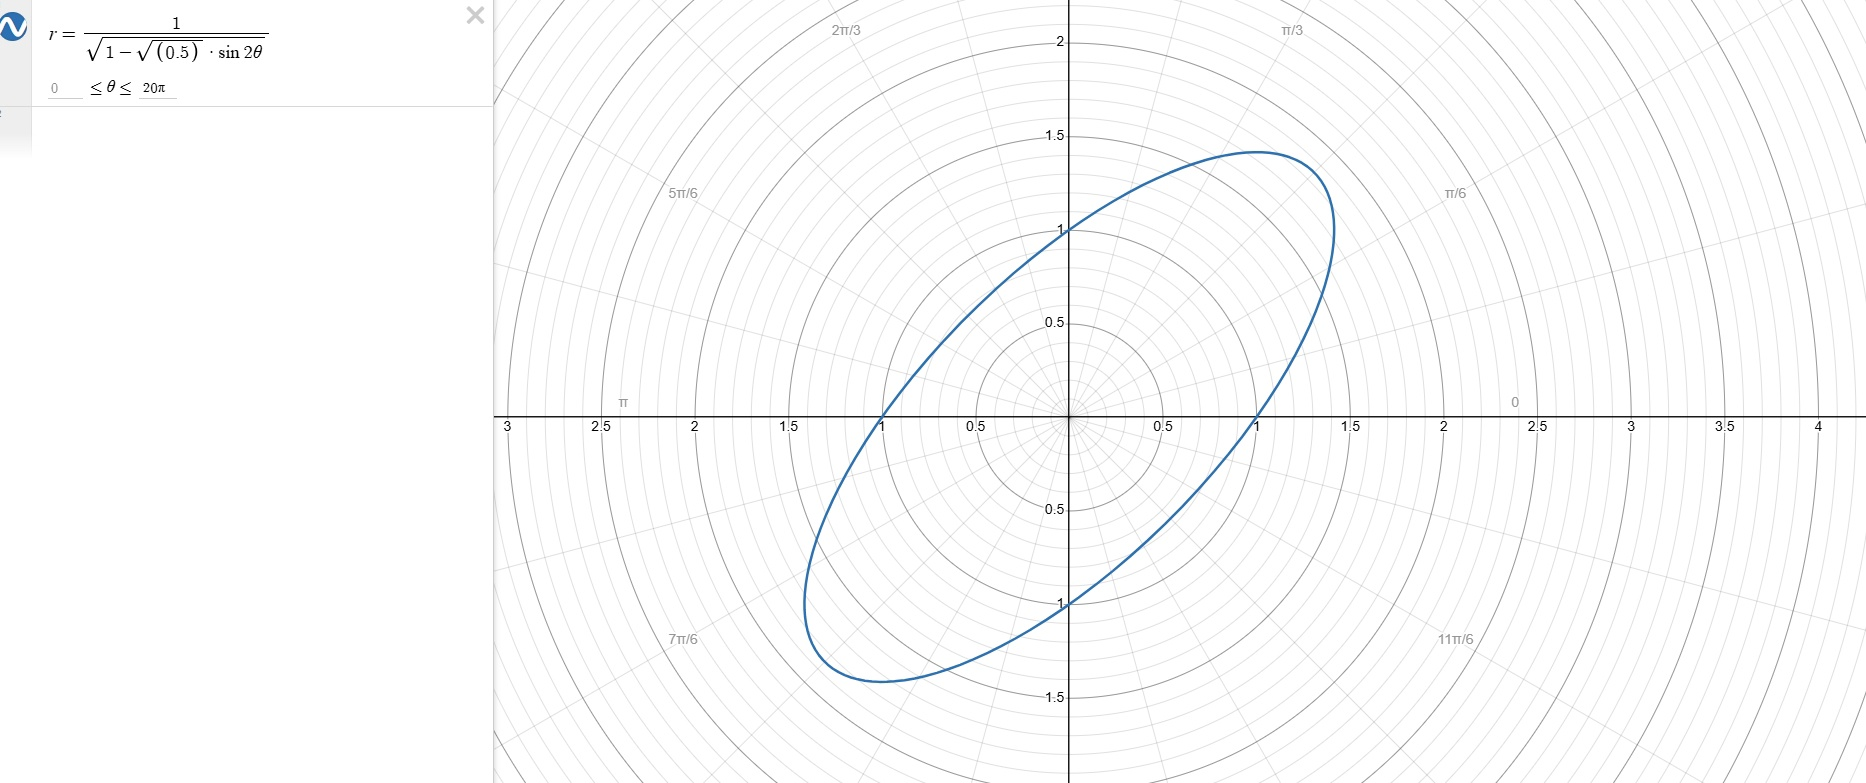
\includegraphics[width=0.7\textwidth]{Graphic3_2.jpg}
    \caption{Траектория 2.}
\end{figure}
\clearpage
\begin{figure}[h]
    \centering
    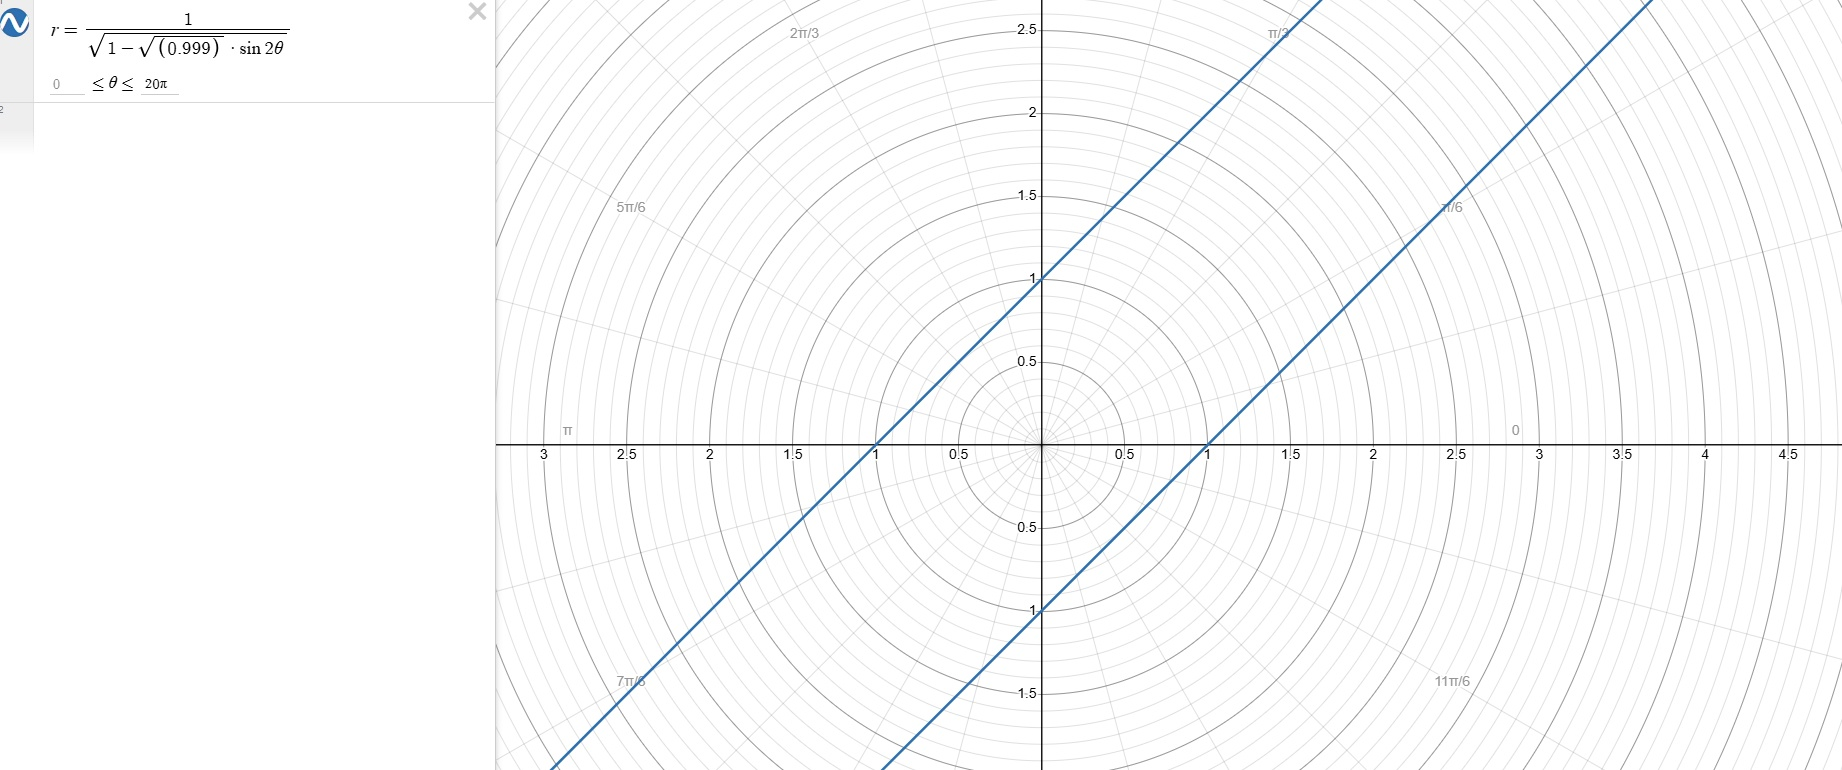
\includegraphics[width=0.7\textwidth]{Graphic3_3.jpg}
    \caption{Траектория 3.}
\end{figure}

Зависимость $\varepsilon(r)$

\[
\frac{{v_{r}}^2}{2} + \frac{2\sigma^2}{r^2} + 2GMr^2 = \varepsilon.
\]

На бесконечности график ведет себя как парабола, вблизи нуля - как гипербола. Продифференцируем по $r$ функцию и найдем точки минимума

\[
\varepsilon'(r) = -\frac{4\sigma^2}{r^2} + 4GMr.
\]

Приравниваем $\varepsilon'(r)$ к 0 и получаем, что $r_{12} = \pm \sqrt[\leftroot{0}\uproot{1}4]{\frac{\sigma^2}{GM}}$

При $\varepsilon = \varepsilon(r_{12})$ траектория будет инфинитной, при $\varepsilon > \varepsilon(r_{12})$ траектория финитная


\begin{figure}[h]
    \centering
    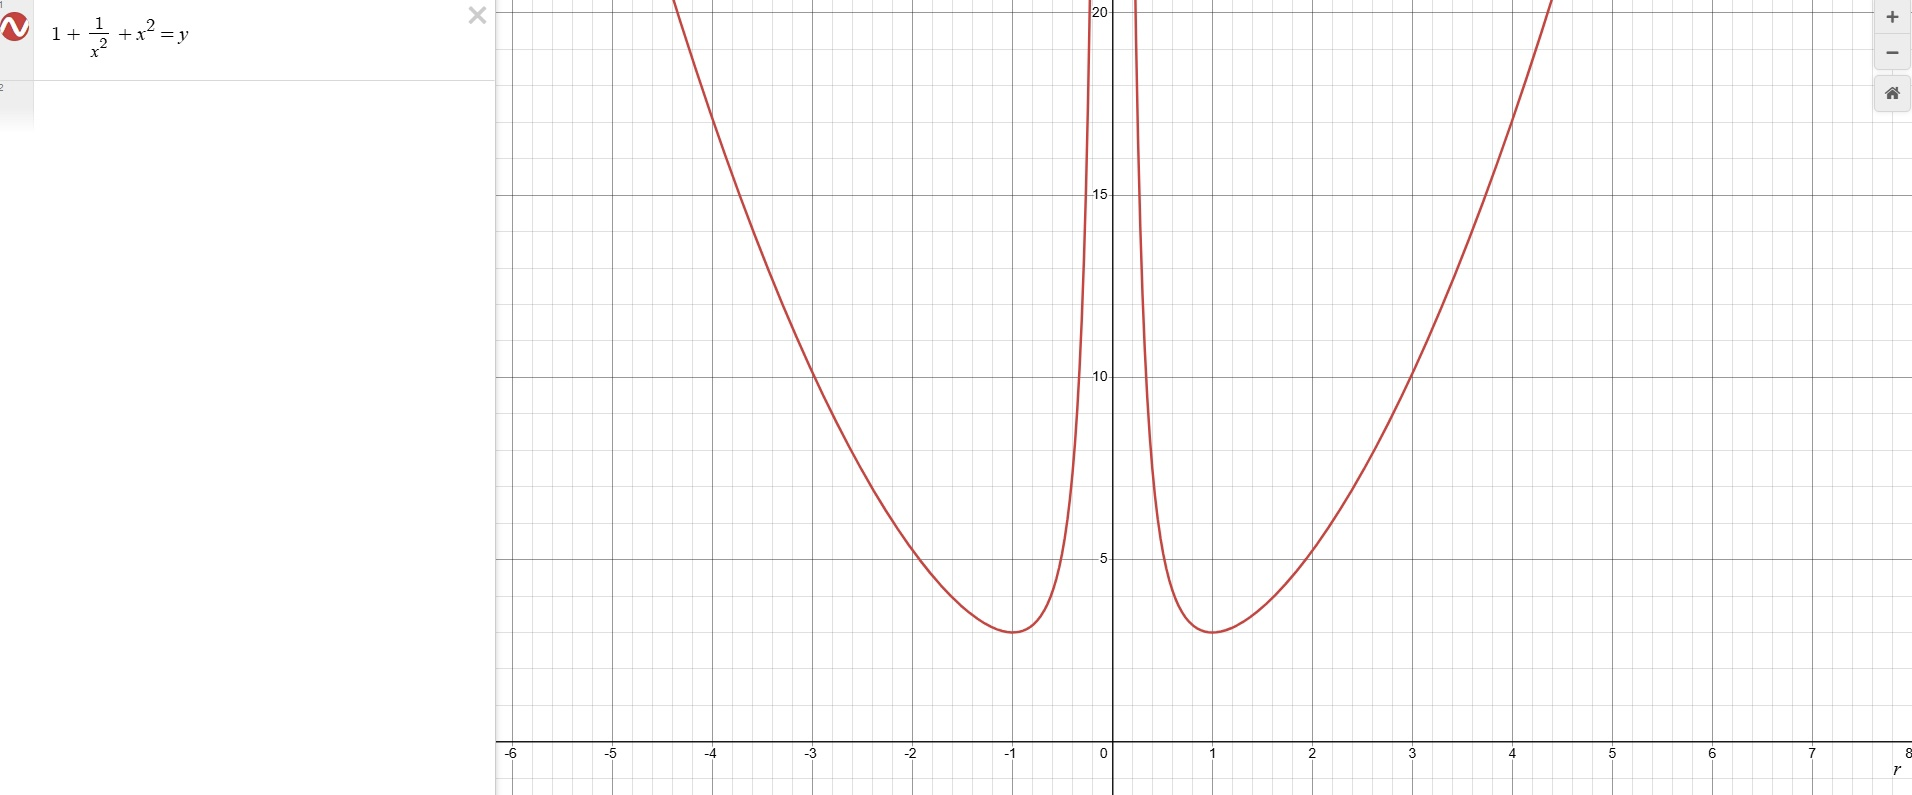
\includegraphics[width=0.9\textwidth]{Finit2.jpg}
    \caption{График $\varepsilon(r) $№2.}
\end{figure}

\section{Отталкивающая сила, обратно пропорциональная кубу расстояния}
Теперь предположим, что гравитационная сила - это сила не притяжения, а отталкивания. Или можно считать, что сила притягивающая, но масса у Солнца отрицательная, и тогда $M$ - модуль массы. Тогда проделаем все те же действия для следующего закона

\[
\vec{F} = \frac{GMm} {r^4} \vec{r}
\]

Потенциальная энергия гравитационного взаимодействия

\[
E_{\text{п}} = \int_{r}^{\infty}{(\vec{F} , d\vec{r})} = \int_{r}^{\infty}{\frac{GMm}{r^3} \, dr} = \frac{2GMm}{r^2}.
\]

Дифференциальное уравнение

\[
(\frac{1}{r^2}\frac{dr}{d\varphi})^2 + \frac{1}{r^2} = \frac{1}{2\sigma^2}(\varepsilon - \frac{2GM}{r^2}),
\]

\[
\int{\frac{dr}{r\sqrt{\varepsilon r^2 - 2GM - 2\sigma^2}}} = \int{\frac{\pm d\varphi}{\sqrt{2}\sigma}},
\]

\[
\frac{\arctg{\frac{\sqrt{\varepsilon r^2-2\sigma^2-2GM}}{\sqrt{2\sigma^2+2GM}}}}{\sqrt{\sigma^2+GM}} = C \pm \frac{\varphi} {\sigma}.
\]

\begin{equation} \tag{9}
r(\varphi) =\pm \frac{\sqrt{\frac{2(\sigma^2+GM)}{\varepsilon}}}{\cos(\varphi_0 \pm \frac{\sqrt{\sigma^2+GM}}{\sigma}\varphi)}.
\end{equation}

Теперь величина $\frac{\sqrt{\sigma^2+GM}}{\sigma} > 1$. Траектория будет выглядеть подобным образом при любых значениях параметров

\begin{figure}[h]
    \centering
    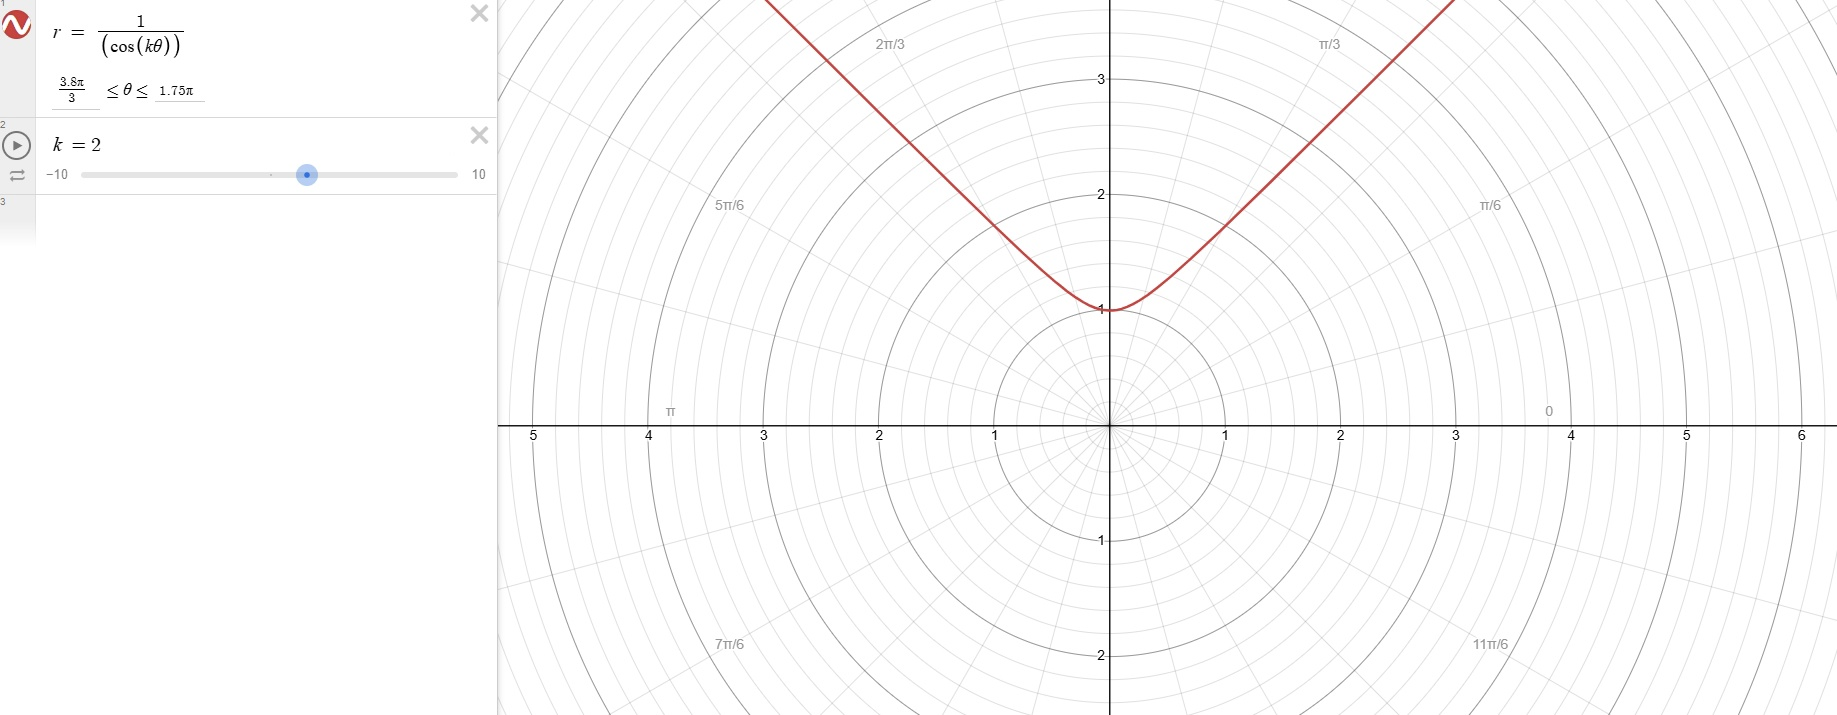
\includegraphics[width=0.9\textwidth]{Graphic4.jpg}
    \caption{Траектория 1.}
\end{figure}

Зависимость $\varepsilon(r)$

\[
\frac{{v_{r}}^2}{2} + \frac{2\sigma^2}{r^2} + \frac{2GM}{r^2} = \varepsilon.
\]

График гиперболы, с ветвями в 1 и 2 четвертях. Траектория всегда инфинитная, что логично

\begin{figure}[h]
    \centering
    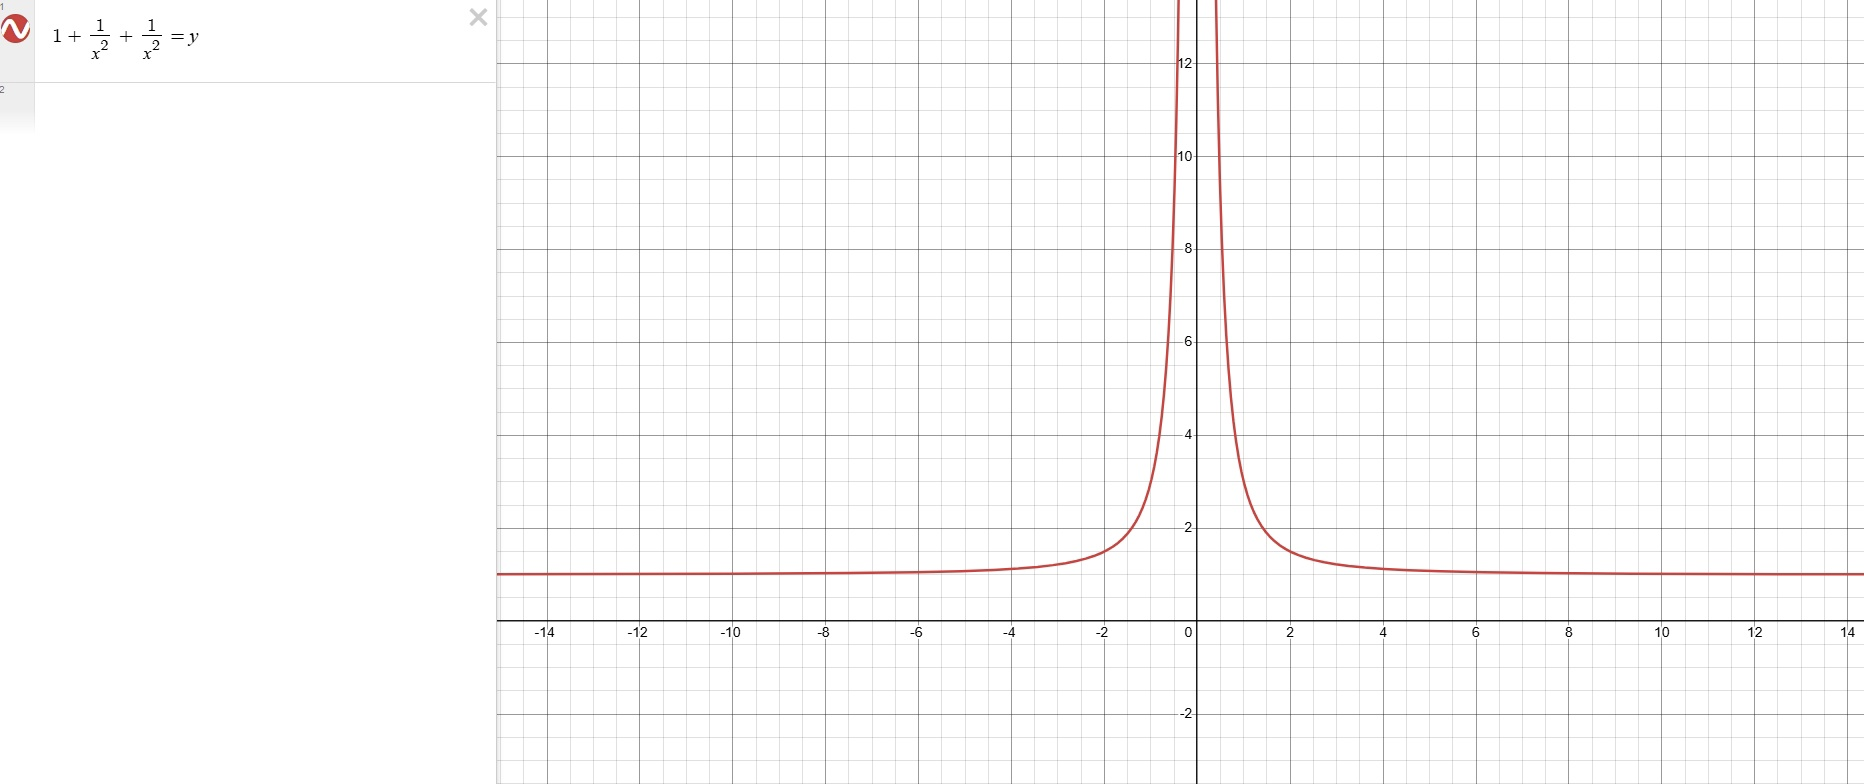
\includegraphics[width=0.9\textwidth]{Finit3.jpg}
    \caption{График $\varepsilon(r) $№3.}
\end{figure}

\section{Отталквающая сила, прямо пропорциональная расстоянию в первой степени}
\[
\vec{F} = GMm \vec{r}.
\]
Потенциальная энергия гравитационного взаимодействия

\[
E_{\text{п}} = \int_{r}^{\infty}{(\vec{F} , d\vec{r})} = \int_{r}^{\infty}{GMmr \, dr} = -2GMm r^2.
\]

Дифференциальное уравнение

\[
(\frac{1}{r^2}\frac{dr}{d\varphi})^2 + \frac{1}{r^2} = \frac{1}{2\sigma^2}(\varepsilon + 2GMr^2),
\]

\[
\int{\frac{dr}{r\sqrt{\varepsilon r^2 + 2GMr^4 - 2\sigma^2}}} = \int{\frac{\pm d\varphi}{\sqrt{2}\sigma}},
\]

\[
\frac{\arcsin{\frac{\varepsilon r^2 - 4\sigma^2}{\sqrt{\varepsilon^2+16GM\sigma^2} r^2}}}{2\sqrt{2}\sigma} = C \pm \frac{\varphi} {\sqrt{2}\sigma}.
\]

Итого

\begin{equation} \tag{10}
r(\varphi) =\pm \frac{\frac{2\sigma}{\varepsilon}}{\sqrt{1-\sqrt{1+\frac{16GM\sigma^2}{\varepsilon^2}}\sin{(\varphi_0 + 2\varphi)}}}.
\end{equation}

При переходе в ДПСК получится гипербола, поскольку $e > 1$.

\begin{figure}[h]
    \centering
    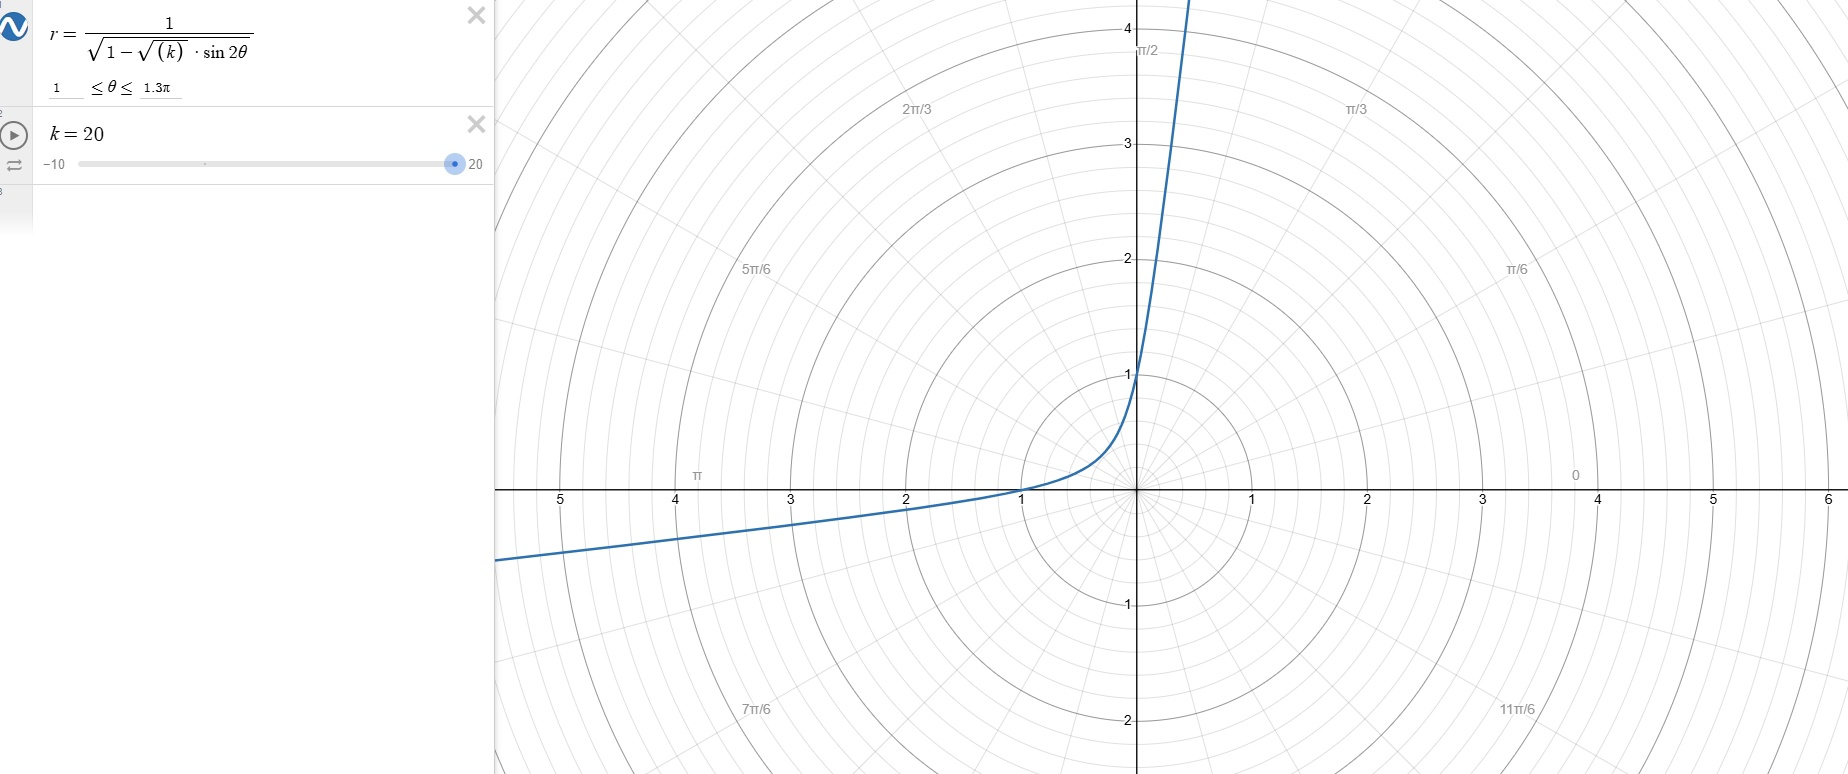
\includegraphics[width=0.9\textwidth]{Graphic5.jpg}
    \caption{Траектория 3.}
\end{figure}

Зависимость $\varepsilon(r)$

\[
\frac{{v_{r}}^2}{2} + \frac{2\sigma^2}{r^2} - 2GMr^2 = \varepsilon.
\]

Аналогично зависимости $\varepsilon(r)$ у силы со знаком "-", но на бесконечности ветви параболы смотрят вниз. Траектория всегда инфинитная
\clearpage
\begin{figure}[h]
    \centering
    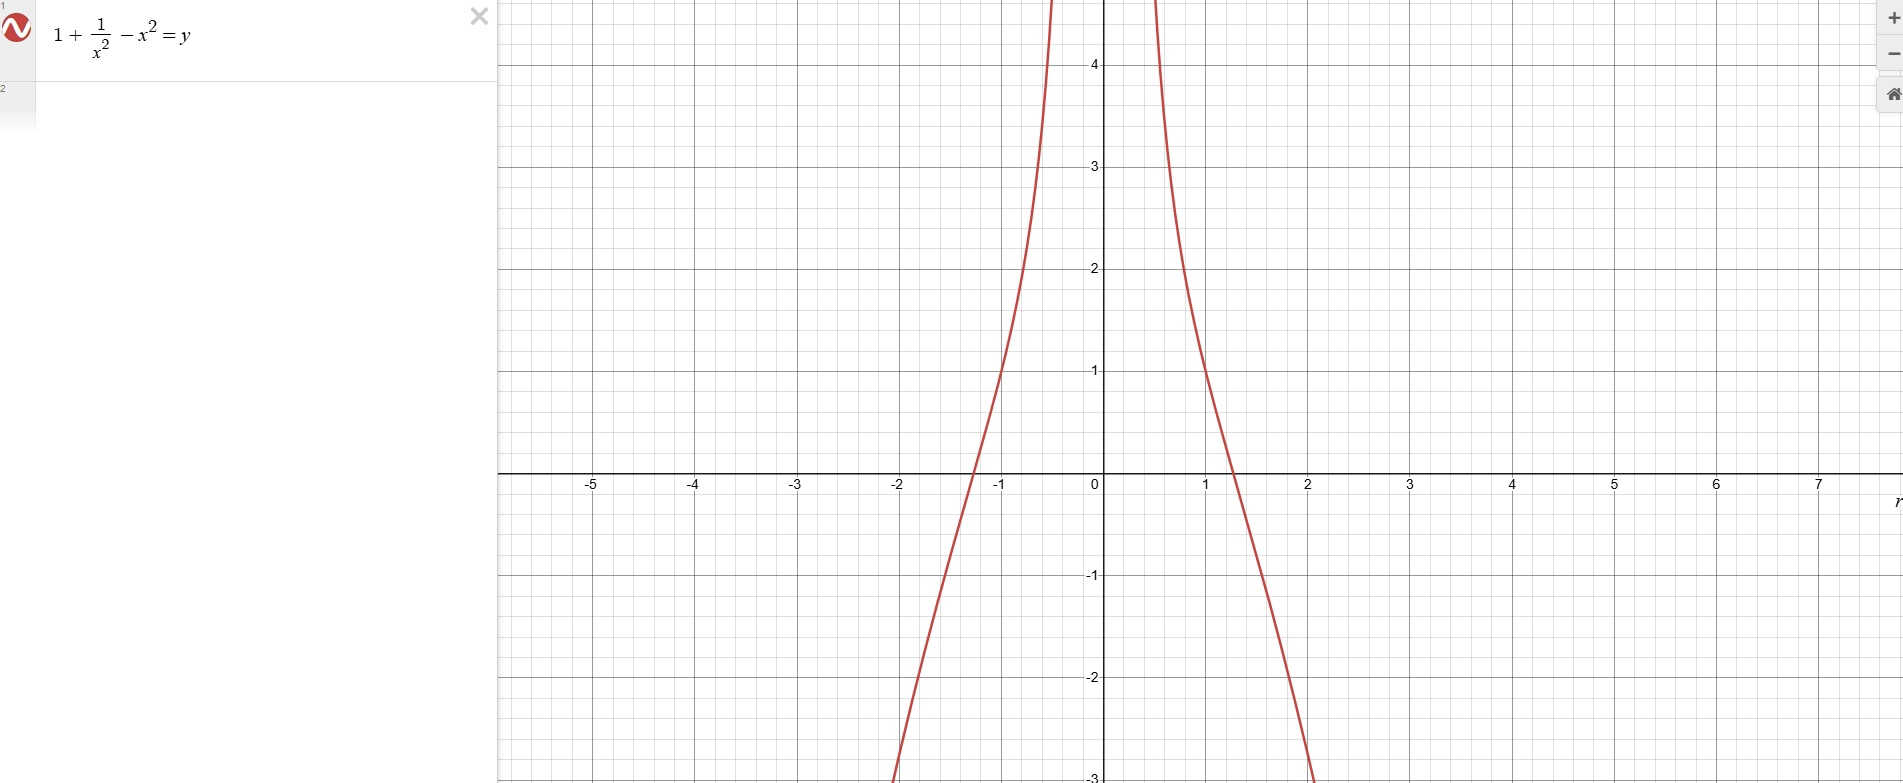
\includegraphics[width=0.9\textwidth]{Finit4.jpg}
    \caption{График $\varepsilon(r) $ №4.}
\end{figure}


\section*{Вывод}
В данной работе были получены уравнения движения небесных тел подчиняющихся как закону Ньютона, так и другим зависимостям. Были построены графики в полярных координатах $r(\varphi)$. Был проведен анализ траекторий с точки зрения графика и алгебры, так и с точки зрения физики.

\end{document}